%******************************************************************************%
%                                                                              %
%                                 Interlude                                    %
%                         for Machine Learning module                          %
%                                                                              %
%******************************************************************************%

% =============================================== %
\section*{Interlude}
% =============================================== %
\subsection*{Regularized Gradient}
% ----------------------------------------------- %
\begin{figure}[!h]
    \centering
    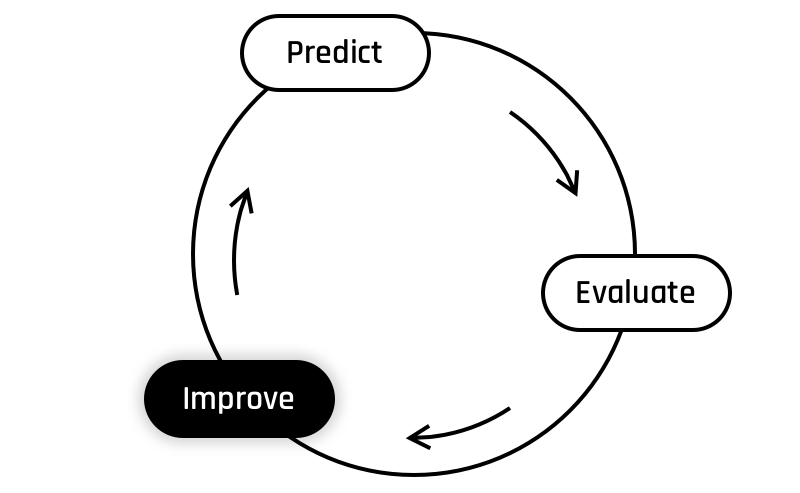
\includegraphics[scale=0.25]{assets/Improve.png}
    %\caption{The Learning Cycle: Improve}
\end{figure}

To derive the gradient of the regularized loss function, $\nabla(J)$ you have to change a bit the formula of the unregularized gradient.  
Given the fact that we are not penalizing $\theta_0$, the formula will remain the same as before for this parameter. For the other parameters ($\theta_1, \dots, \theta_n$), we must add the partial derivative of the regularization term: $\lambda \theta_j$.

Therefore, we get:
$$
\nabla(J)_0 = \frac{1}{m}\sum_{i=1}^{m}(h_\theta(x^{(i)}) - y^{(i)})
$$
$$
\nabla(J)_j = \frac{1}{m}\left(\sum_{i=1}^{m}(h_\theta(x^{(i)}) - y^{(i)})x_j^{(i)} + \lambda \theta_j\right) \text{ for j = 1, ..., n}
$$

Where:  
\begin{itemize}
    \item $\nabla(J)_j$ is the j$^\text{th}$ component of the gradient vector $\nabla(J)$,
    \item $m$ is the number of training examples used,
    \item $h_\theta(x^{(i)})$ is the model's prediction for the i$^\text{th}$ training example,
    \item $x^{(i)}$ is the feature vector of the i$^\text{th}$ training example,
    \item $y^{(i)}$ is the expected target value for the i$^\text{th}$ example,
    \item $\lambda$ is a constant, the regularization hyperparameter,
    \item $\theta_j$ is the j$^\text{th}$ parameter of the $\theta$ vector.
\end{itemize}

Which can be vectorized as:
$$
\nabla(J) = \frac{1}{m} [X'^T(h_\theta(X) - y) + \lambda \theta']
$$  

Where:  
\begin{itemize}
    \item $\nabla(J)$ is a vector of dimension $(n + 1)$ the gradient vector,
    \item $m$ is the number of training examples used,
    \item $X$ is a matrix of dimension $(m \times n)$, the design matrix,
    \item $X'$ is a matrix of dimension $(m \times (n + 1))$, the design matrix onto which a column of ones is added as a first column,
    \item $y$ is a vector of dimension $m$, the vector of expected values,
    \item $h_\theta(X)$ is a vector of dimension $m$, the vector of predicted values,
    \item $\lambda$ is a constant,
    \item $\theta$ is a vector of dimension $(n + 1)$, the parameter vector,
    \item $\theta'$ is a vector of dimension $(n + 1)$, constructed using the following rules:
\end{itemize}

$$
\begin{matrix}
\theta'_0 & =  0 \\
\theta'_j & =  \theta_j & \text{ for } j = 1, \dots, n\\    
\end{matrix}
$$

% =============================================== %
\subsection*{Linear Gradient vs Logistic Gradient}
% ----------------------------------------------- %
As before, we draw your attention on the only difference between linear regression and logistic regression's gradient equations: \textbf{the hypothesis function} $h_\theta(X)$.
\begin{itemize}
    \item In the linear regression: $h_\theta(X) = X'\theta$,
    \item In the logistic regression: $h_\theta(X) = \text{sigmoid}(X'\theta)$.
\end{itemize}
